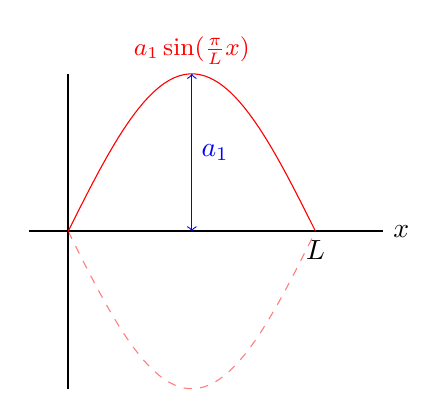
\begin{tikzpicture}
% Axis
\draw[thick] (-.5,0)--(4,0) node[right]{$x$};
\draw[thick] (0,-2)--(0,2) node[above]{ };

\draw[red, samples=50, domain=0:pi] plot ({\x},{2*sin( \x r)});
\draw[red, samples=50, domain=0:pi, dashed, opacity=0.5] plot ({\x},{2*-sin( \x r)});

\node[above, red] at (pi/2,2) {\small $a_1 \sin(\frac{\pi}{L}x)$};

\draw[<->,blue, samples=50] (pi/2,0) -- (pi/2,2) node[right, pos=0.5]{$a_1$};

\node[below] at (pi,0) {$L$};

\end{tikzpicture}
